\documentclass{./../div_teaching_slides}

\begin{document}
\title{ECON 340 \\ Economics Research Methods}
\author{Div Bhagia}
\date{Midterm Review}

\begin{frame}[noframenumbering, plain]
\maketitle
\end{frame}

%%%%%%%%%%%%%%%%%%%%
\begin{frame}{Midterm Exam}
\begin{witemize}
	\item 1 hour 10 minutes, 20 points 
	\item Closed book, can use a calculator 
	\item Formula sheet and Normal Distribution table will be provided 
	\item Study guide, formula sheet, and sample midterm is uploaded on Canvas \\~\\
\end{witemize}

\textit{Next week}: No class on Tuesday. Instead, we will have research project meetings. 
\end{frame}

%%%%%%%%%%%%%%%%%%%%
\begin{frame}{Topics covered}
\vspace{-0.85em}
\begin{itemize}
\item Summation notation
\item Describing Data \\ 
\begin{itemize}
\item Frequency distribution
\item Mean, median, variance, standard deviation 
\item Add. topics: Percentiles, weighted mean, z-score
\item Covariance and correlation
\end{itemize}
\item Random variables \\
\begin{itemize}
\item Expected value and variance 
\item Normal and standard normal distribution
\item Conditional expectation, uncorrelatedness and independence
\end{itemize}
\item Sampling and Estimation \\
\begin{itemize}
\item Sample mean distribution, CLT
\item Properties of a good estimator
\item Confidence intervals, hypothesis tests, p-values
\end{itemize}
\end{itemize}
\end{frame}

%%%%%%%%%%%%%%%%%%%%
\begin{frame}{Mean}
Sample mean:
$$ \bar{X} = \frac{1}{n}\sum_{i=1}^n X_i $$ \\~\\
The population mean is denoted by $\mu$. \\~\\
For grouped data:
 $$ \bar{X} =\frac{1}{n} \sum_{k=1}^J n_k X_k = \sum_{i=1}^J f_k X_k $$ 
 Example: $X_i: 2, 2, -4, 2$
\end{frame}

%%%%%%%%%%%%%%%%%%%%
\begin{frame}{Variance}
Population variance:
$$ \sigma_X^2 = \frac{1}{N} \sum_{i=1}^N (X_i-\mu_X)^2 $$ \\
\vspace{0.5em}
Sample variance:
$$ S_X^2 = \frac{1}{n-1} \sum_{i=1}^n (X_i-\bar{X})^2 $$ \\
\vspace{0.5em}
Standard Deviation
$$ \sigma_X = \sqrt{\sigma_X^2} \quad \quad S_X = \sqrt{S_X^2} $$ \\
\end{frame}

%%%%%%%%%%%%%%%%%%%%
\begin{frame}{Variance: Grouped Data}
Alternatively, population variance:
$$ \sigma_X^2 = \sum_{k=1}^J f_k (X_k-\mu_X)^2 $$  \\
\vspace{1cm}
Sample variance:
$$ S_X^2 = \frac{n}{n-1} \sum_{k=1}^J f_k (X_k-\bar{X})^2 $$
\end{frame}

%%%%%%%%%%%%%%%%%%%%
\begin{frame}{The variance of $Y$ is higher in which plot?}
\begin{columns}
\begin{column}{0.475\textwidth}
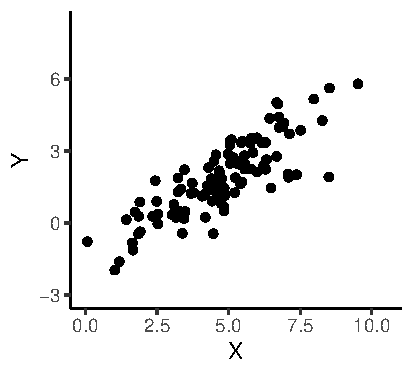
\includegraphics{./../../Output/review_scatter1}
\end{column}
\begin{column}{0.475\textwidth}
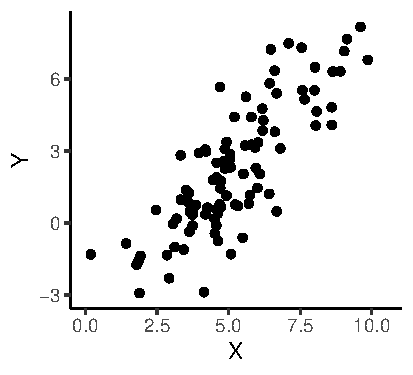
\includegraphics{./../../Output/review_scatter2}
\end{column}
\end{columns}
\end{frame}

%%%%%%%%%%%%%%%%%%%%
\begin{frame}{Weighted Mean}
Weighted mean:
$$ \bar{X}^{\omega} = \frac{\sum_{i=1}^n\omega_i X_i}{\sum_{i=1}^n \omega_i} $$
where $\omega_i$ is the weight of the $i^{th}$ observation. \\~\\ When weights sum up to 1 (i.e. \(\sum_{i=1}^n \omega_i=1\)) we can simply write the weighted mean as:
$$ \bar{X} = \sum_{i=1}^n\omega_i X_i$$ 
\end{frame}	

%%%%%%%%%%%%%%%%%%%%
\begin{frame}{Example}
\vspace{-0.5em}
\begin{witemize}
	\item We want to estimate the average starting salary of students at a university that has only two majors	\item Half of the students are \textit{Business} majors, while the other half are \textit{Engineering} majors
	\item Randomly select 100 Business students and 100 Engineering for a survey
	\item Response rate among Business students is 100\%, while it 50\% for engineering students 
	\item[] \textit{How can we use weighting to adjust for this?}
\end{witemize}
\end{frame}	

%%%%%%%%%%%%%%%%%%%%
\begin{frame}{Covariance}
	$$ \sigma_{XY} = \frac{1}{N}\sum_{i=1}^N (X_i-\mu_X)(Y_i-\mu_Y) \quad (Population) $$
	\vspace{1em}
$$ S_{XY} = \frac{1}{n-1}\sum_{i=1}^n (X_i-\bar{X})(Y_i-\bar{Y}) \quad (Sample) $$ 

\vspace{1cm}
Why does the formula work?
\end{frame}

%%%%%%%%%%%%%%%%%%%%
\begin{frame}{Scatterplot}
\centering
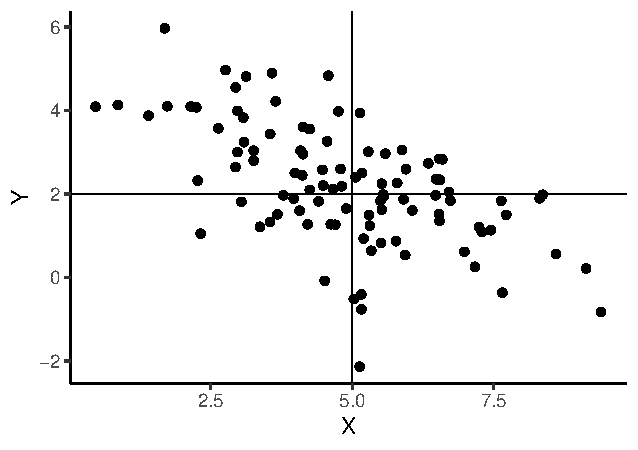
\includegraphics{./../../output/corr_midterm}
\end{frame}

%%%%%%%%%%%%%%%%%%%%
\begin{frame}{Correlation}
$$ \rho_{XY} = \frac{ \sigma_{XY}}{\sigma_X \sigma_Y}  \quad (Population) $$ \\
\vspace{1em}
$$ r_{XY} = \frac{ S_{XY}}{S_X S_Y} \quad (Sample) $$

\vspace{1cm}
Why use correlation instead of covariance?
\end{frame}

%%%%%%%%%%%%%%%%%%%%
\begin{frame}{Correlation}
	\begin{itemize}
\item Measures the strength and direction of the linear relationship between two variables
\item Bounded between -1 and 1
\item If zero, there is no linear relationship. If 1 or -1 perfect linear relationship.
\item If negative, when $X$ is above (below) $\bar{X}$, $Y$ tends to be above (below) $\bar{Y}$.
\item If negative, when $X$ is above (below) $\bar{X}$, $Y$ tends to be below (above) $\bar{Y}$.
\end{itemize}
\end{frame}

%%%%%%%%%%%%%%%%%%%%
\begin{frame}{Correlation is not causation!}
A positive correlation between job vacancies and immigration doesn’t
suggest that immigration $\rightarrow$ job creation. Why? \\~\\
\begin{witemize}
\item[1.] \textit{Reverse causality:} jobs $\rightarrow$ immigration
\item[2.] \textit{Other confounding factors:} government policies $\rightarrow$ jobs, government policies $\rightarrow$ immigration   
\end{witemize}
\end{frame}

%%%%%%%%%%%%%%%%%%%%
\begin{frame}{Random Variables}
	A random variable is a variable that takes different values under different scenarios. Used for modeling uncertain outcomes.\\~\\
	Discrete RVs: Countable possible values \\
	$$ f(x) = Pr(X=x) $$ \\
	
\vspace{1em}	
Continuous RVs: Any value in an interval 
$$ Pr(a \leq X \leq b) =  \int_{a}^{b} f(x) \partial x $$
\end{frame}

%%%%%%%%%%%%%%%%%%%%
\begin{frame}{Normal Distribution}
\centering \vspace{1em}
\begin{columns}[c]
\begin{column}{0.475\textwidth}
$$ Pr(X\leq 150) $$
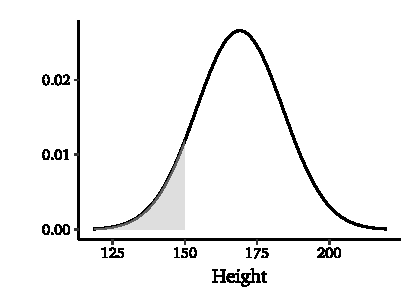
\includegraphics{./../../Output/height_norm2_ho2}
\end{column}
\begin{column}{0.475\textwidth}
$$ Pr(150<X<175) $$
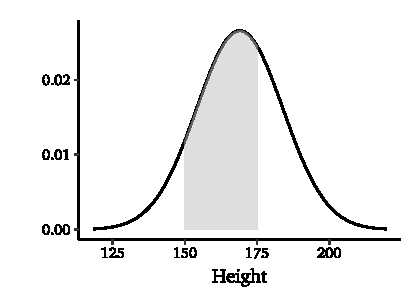
\includegraphics{./../../Output/height_norm2_ho}
\end{column}
\end{columns}
\end{frame}

%%%%%%%%%%%%%%%%%%%%
\begin{frame}{Expectation \& Variance }
Discrete RV:
$$ E(X) = \mu_X= \sum_x x f(x) $$

\vspace{1em}
Continuous RV:
$$ E(X) = \mu_X= \int_x x f(x) \partial x $$

\vspace{1em}
Variance:
$$ Var(X) = \sigma_X^2 = E [(X-\mu_X)^2] $$ 
\end{frame}

%%%%%%%%%%%%%%%%%%%%
\begin{frame}{Example}
You estimate that the price of a stock will increase by 10\% with a probability of 0.6 and decrease by 5\% with a probability of 0.4. Calculate the expected return on the stock and its variance. 
\end{frame}

%%%%%%%%%%%%%%%%%%%%
\begin{frame}{Covariance and Correlation}
Covariance is a measure of the extent to which two random variables move
together. \\~\\
Let $X$ and $Y$ be a pair of random variables, then the \textit{covariance} of $X$ and $Y$ is given by:
$$ \sigma_{XY} = Cov(X,Y) = E[(X-\mu_X)(Y-\mu_Y)] = E(XY)-\mu_X \mu_Y $$ 
\vspace{0.15em}

The \textit{correlation} between $X$ and $Y$ is given by:
$$ \rho_{XY} = corr(X,Y) = \frac{Cov(X,Y)}{\sigma_X \sigma_Y} \quad \text{ where } -1 \leq \rho \leq 1$$
\end{frame}

%%%%%%%%%%%%%%%%%%%%%
%\begin{frame}{Example: Two Stocks}
%\begin{tabularx}{\textwidth}{P{2cm}P{1.25cm}P{1.25cm}P{1.25cm}Y}
%\toprule
%Scenarios ($Z$) & $Pr(Z)$ & 	$X$ & $Y$ & $(X-\mu_X)(Y-\mu_Y)$  \\ \hline
%1 & 0.6 & 10 & -5 \\
%2 & 0.4 & -5 & 10 \\
%\bottomrule 
%\end{tabularx} 
%$$ \mu_X = E(X) = 0.6 \times 10 + 0.4 \times (-5) =6-2 = 4 $$
%$$ \mu_Y = E(Y) = 0.6 \times (-5) + 0.4 \times 10 =-3+4 = 1 $$ 
%
%$$ Cov(X,Y) = E[(X-\mu_X)(Y-\mu_Y)] = \hspace{6cm}  $$
%\end{frame}

%%%%%%%%%%%%%%%%%%%%
\begin{frame}{Conditional Distribution}
The distribution of a random variable $Y$ conditional on another random variable $X$ taking on a specific value is called the conditional
distribution of $Y$ given $X$.
$$ Pr(Y=y| X=x) = \frac{Pr(X=x, Y=y)}{Pr(X=x)}   $$ \\~\\

\textit{Example}: Q2, Problem Set 3
\end{frame}

%%%%%%%%%%%%%%%%%%%%
\begin{frame}{Conditional Expectation}
The \textit{conditional expectation} of $Y$ given $X$ is the mean of the conditional distribution of $Y$ given $X$. \\~\\
$$ E(Y|X=x) = \sum_{y} y Pr(Y=y | X=x) $$
\end{frame}

%%%%%%%%%%%%%%%%%%%%
\begin{frame}{Example}
$X$: Hours spent studying each week, $Y$: exam score \\~\\
What does the following imply?
$$ E(Y|X) = E(Y)  $$
\vspace{0.1em}

What if?
$$ E(Y|X=5) > E(Y|X=1)  $$
\end{frame}

%%%%%%%%%%%%%%%%%%%%
\begin{frame}{Z-score}
Z-score is defined as:
$$ Z = \frac{X - \mu}{\sigma} $$ 

\vspace{1em}
Z-score tells us how many standard deviations any particular observation is away from the mean. \\~\\
So if $X \sim N(\mu, \sigma^2/n)$, what is the distribution of $Z$? \\~\\
\end{frame}

%%%%%%%%%%%%%%%%%%%%
\begin{frame}{Expectation and Variance of $\bar{X}$}
Let $X_1,X_2,...,X_n$ denote independent random draws (random sample) from a population with mean $\mu$ and variance $\sigma^2$. 
$$ \bar{X} = \frac{1}{n} \sum_{i=1}^n X_i $$
The expectation and variance of the sample mean:
$$E(\bar{X}) = \mu \quad \quad Var(\bar{X}) = \sigma^2_{\bar{X}} = \frac{\sigma^2}{n} $$ 
\end{frame}

%%%%%%%%%%%%%%%%%%%%
\begin{frame}{Distribution of the Sample Mean}
What is the shape of the distribution for the sample mean? \\~\\
It is normal when:
\begin{enumerate}
\item The underlying population is normal, or
\item The sample size is large, say $n\geq 100$, by the Central Limit Theorem 
\end{enumerate}
\end{frame}

%%%%%%%%%%%%%%%%%%%%
\begin{frame}{Confidence Intervals}
\begin{witemize}
  \item If $\bar{X} \sim N(\mu, \sigma^2_{\bar{X}})$, can create confidence intervals
  \item To create a 95\% confidence interval, note:
  $$ Pr(-1.96 < Z < 1.96) = 0.95 $$
  \item Since $Z=\frac{\bar{X} - \mu}{\sigma_{\bar{X}}}$, we have
  $$ Pr(\mu-1.96 \sigma_{\bar{X}} < \bar{X} < \mu + 1.96 \sigma_{\bar{X}}) = 0.95 $$
  \item Which implies that:
  $$ Pr(\bar{X}-1.96 \sigma_{\bar{X}} < \mu < \bar{X} + 1.96 \sigma_{\bar{X}}) = 0.95 $$
\end{witemize}
\end{frame}

%%%%%%%%%%%%%%%%%%%%
\begin{frame}{Confidence Intervals}
Let $z_{\alpha/2}$ be the $z$-value that leaves area $\alpha/2$ in the upper tail of the normal distribution. \\~\\
Then $1-\alpha$ confidence interval is given by 
$$ \bar{x} \pm {z_{\alpha/2}  \frac{\sigma}{\sqrt{n}}}$$

Note that, $\sigma_{\bar{X}} = \dfrac{\sigma}{\sqrt{n}}$
\end{frame}

%%%%%%%%%%%%%%%%%%%%
\begin{frame}{Hypothesis Testing: Recipe}
1. Set up the null and alternative hypotheses:
$$ H_0: \mu = \mu_0 \quad \quad H_1: \mu \neq \mu_0$$ \\~\\
2. Calculate test statistic:
$$z =  \frac{\bar{X} - \mu_0}{\sigma/\sqrt{n}}$$ \\~\\
3. Reject the null if $|z|>z_{\alpha/2}$
\end{frame}

%%%%%%%%%%%%%%%%%%%%
\begin{frame}{p-Value}
The p-value is defined as the probability of randomly drawing an outcome this surprising or even more surprising given the null hypothesis. \\~\\
$$ p = 2 P(Z>|z|) $$

\vspace{1cm}
If $p$-value $ <\alpha$, we reject the null.

\end{frame}

%%%%%%%%%%%%%%%%%%%%
\begin{frame}{When we don't know $\sigma^2$}
	Don't know the true population variance $\sigma^2$, use sample variance $S^2$. \\~\\ 
	The resulting test statistic:
	$$ T = \frac{\bar{X}-\mu_0}{S/\sqrt{n}} \sim t_{n-1} $$ 
follows a $t$ distribution with $n-1$ degrees of freedom. \\~\\
In large samples, say $n \geq 100$, $t$ is identical to standard normal so you can still refer to the standard normal table for critical values. 
\end{frame}

%%%%%%%%%%%%%%%%%%%%
\begin{frame}{Example}
\vspace{-0.1cm} \small
A university wants to test whether online classes yield similar exam scores to in-person classes. Historically, the average exam score for traditional classes has been 75. A random sample of 100 exam scores from online classes reveals an average score of 71.5 with a standard deviation of 20. \\  \vspace{0.1cm}
\begin{itemize}
  \item Test the hypothesis that scores from online classes are significantly different from in-person classes at a 10\% level of significance.
  \item What is the $p$-value associated with your hypothesis test?
  \item What about testing this hypothesis at a 5\% level of significance?
  \item Create a 95\% confidence interval for average score from online classes.
\end{itemize}

\end{frame}

%%%%%%%%%%%%%%%%%%%%
\begin{frame}
\vfill \centering \huge
\purple{Good luck!}
\vfill
\end{frame}

\end{document}